\chapter{The Standard Model and Beyond}
%\addcontentsline{toc}{chapter}{Introduction}

\section{The Standard Model}

Four basic forces mediate all known interactions among the particles of matter \cite{t_hooft_gauge_1980}. Electromagnetic and gravitational are infinite range forces, so they are familiar to everyone for their macroscopic effects. The two remaining forces, which are called the weak and the strong force, cannot be perceived directly because their influence extends no larger than the radius of an atomic nucleus. The strong force binds together the protons and neutrons in the nucleus, and glues the quarks to constitute hadrons. The weak force is mainly responsible for decay processes, characterized by a long lifetime and the large mass of the weak bosons that carry the interaction; the typical lifetime of particles decaying via strong interaction is $\sim 10^{-23}$ seconds, while decays via weak interaction can take $\sim 10^{-12}$ seconds or longer \cite{Halzen:1984mc}.

The standard model (SM) \cite{Novaes:1999yn} of elementary particles describes the nature of the forces by means of non-abelian gauge theories \cite{Quigg:2013ufa}. Electromagnetic and weak forces are mediated by the gauge particles of the Glashow--Weinberg--Salam model \cite{Glashow:1961tr}, namely the massless photon and a triplet of massive vector bosons, the $W^+,W^{-}$, and $Z^0$. The strong force is attributed to the eight massless gluons of quantum chromodynamics. In addition, there is one scalar Higgs boson, which is massive and electrically neutral. These quantum field theories incorporate quantum mechanics and special relativity to describe three of the four fundamental interactions: strong, electromagnetic, and weak interactions. The gravitational interaction is far weaker and is not expected to contribute significantly to any processes at subatomic level.

The fundamental particles  of matter are six leptons and six flavors of quarks, each of the quarks being present in three colors (Fig. \ref{smplot}). There exist 12 fermions (6 quarks plus 6 leptons), 4 vector bosons ($W, Z$, photon, gluon), and one scalar field (Higgs) responsible for the mechanism of electroweak symmetry breaking (EWSB). Each particle has its own anti-particle related by charge conjugation. 

\begin{figure}[hb!!]
\centering
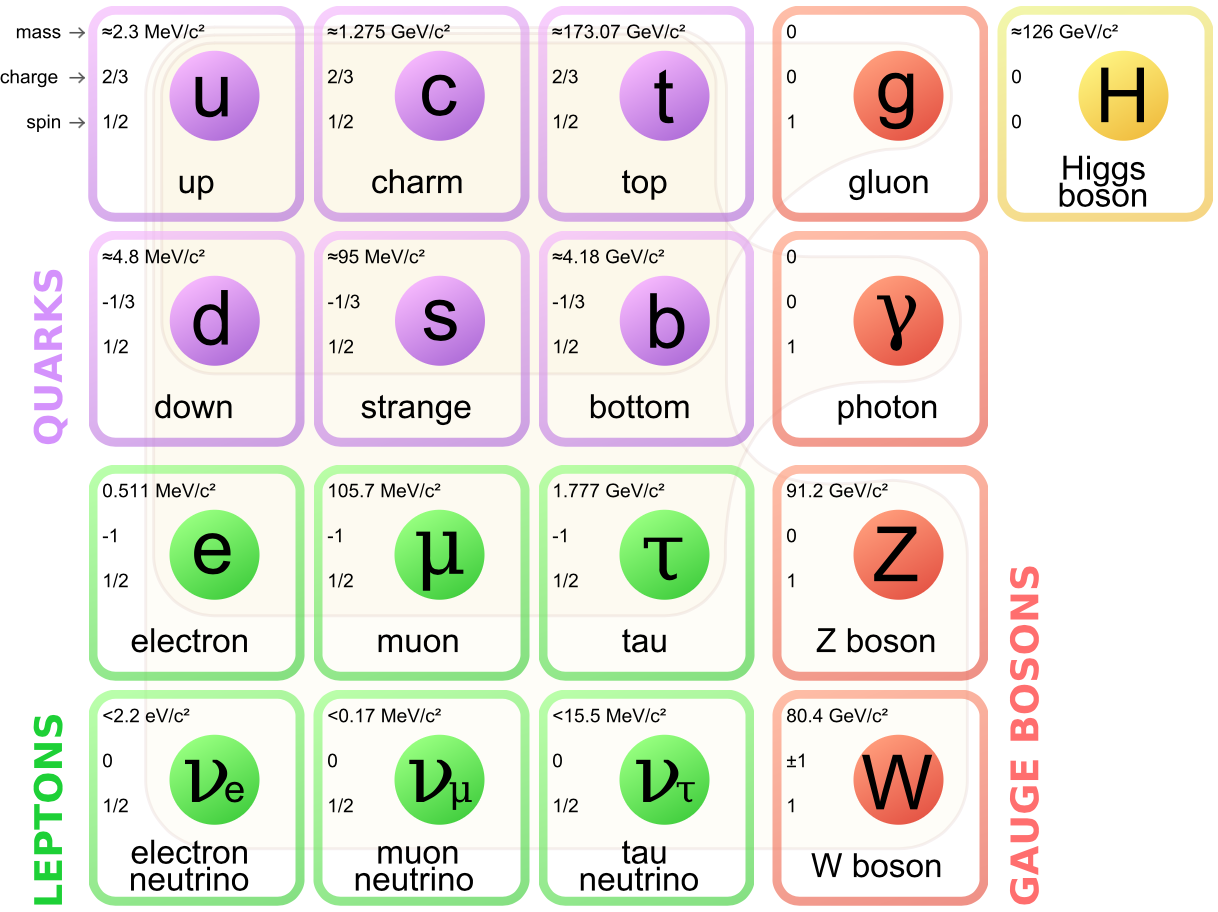
\includegraphics[scale=0.2]{figures/theory/standard.png}
\caption[Elementary particles in the standard model]{The standard model of elementary particles with three generations of quarks and leptons, gauge bosons, and the Higgs boson. [\href{http://tinyurl.com/loorj2q}{public domain}]}
\label{smplot}
\end{figure}

Quarks are the constituents of composite particles called hadrons, which are bound states of quark--antiquark for the case of mesons ({\it e.g.}, $\pi^+, \pi^-, \pi^0$, etc.), or three--quark states for the case of baryons ({\it e.g.}, protons, neutrons, $\Delta^{++}$, etc.). Single quark states cannot be observed as free particles, have fractional electric charge, and a quantum number called ``color'', which is the source of the strong interaction. Gluons, the mediators of color flow in the strong interactions, carry eight combinations of color and anti-color. 

Leptons, having the electron as the best known member, do not undergo strong interactions because they do not carry color. Besides the charged leptons, there are neutral leptons: the neutrinos. Neutrinos only interact via the weak force, consequently, their detection in collider experiments is usually inferred by energy imbalance in a specific reaction. 

\subsubsection*{Gauge Symmetry}

Gauge invariance is the mechanism that determines the dynamical forces among the fundamental constituents of matter \cite{Pich:2012sx}. The fields associated with the elementary particles are representations of a symmetry group; for the standard model, the governing symmetry group is
\begin{equation}
SU(3)_C \times SU(2)_L \times U(1)_Y\,. \label{group}
\end{equation}
The factor $SU(3)_C$ corresponds to the strong sector, carries the color charge, and generates $(3^2-1)$ gauge fields associated with the eight gluons. The factor $SU(2)_L\times U(1)_Y$ corresponds to the electroweak sector, carries isospin and hypercharge, and generates $(3+1)$ gauge fields associated with the weak bosons and the photon.

\subsection{Strong Sector}
Quantum chromodynamics (QCD) is the theory of the strong interactions between quarks and gluons, governed by the symmetry group $SU(3)_C$. The fundamental representation of $SU(3)_C$ is a triplet, so the three quark colors red, green, and blue, or $(r, g, b)$, form the fundamental representation:
\begin{equation}
q = \left(\begin{array}{c} q^r\\ q^g\\ q^b \end{array} \right)\,.
\end{equation}
In this representation, the $SU(3)_C$ generators are the Gell-Mann matrices denoted $\lambda^a$, with $a=1,\ldots ,8$. The QCD Lagrangian is given by
\begin{equation}
\lagrangean_{QCD}=\sum_{q=u,d,s\ldots}\!\!\bar{q}(i\not\!\!D - m_q)q \: - \: \frac{1}{4}G_{\mu\nu}^a G^{a\mu\nu}
\label{Lqcd}
\end{equation}
where the sum runs over the quark flavors up ($u$), down ($d$), strange ($s$), charm ($c$), bottom ($b$), and top ($t$). The strength tensor of the gluon field $G_\mu^a$ is given by
\begin{equation}
G_{\mu\nu}^a = \partial_\mu G_\nu^a-\partial_\nu G_\mu^a-g_s f^{abc}G_\mu^bG_\nu^c
\end{equation}
where the structure constant $f^{abc}$ of the $SU(3)_C$ group is defined through 
\begin{equation}
[\lambda^a,\lambda^b]=2if^{abc}\lambda^c \; . 
\end{equation}

\noindent The covariant derivate is defined as
\begin{equation}
D_\mu q = \Bigl(\partial_\mu +ig_s\frac{\lambda^a}{2}G_\mu^a\Bigr)q
\end{equation}
where $g_s$ is the coupling of the strong force. 

The strong interactions have a characteristic energy scale $\Lambda\sim 200$ MeV interpreted as the energy at which the coupling constant diverges. The running of the coupling constant obtained by the renormalization group equation at leading order of perturbation theory is given by
\begin{equation}
\alpha_S(Q^2) = \frac{12\pi}{(33-2n_f)\log(Q^2/\Lambda^2)}
\end{equation}
where $n_f$ is the number of quark flavors and $Q^2$ the probed energy. At very large $Q^2$, corresponding to small distances, $\alpha_S = g_s/4\pi$ becomes increasingly small. This phenomena is known as asymptotic freedom, property that allows perturbative expansion at small distances.

\subsection{Electroweak Sector}
The 12 fundamental fermions are grouped in three generations:
\begin{equation*}
\left\lbrace
\begin{array}{cc}
\nu_e & u \\
e     & d
\end{array}
\right\rbrace \,,\quad
\left\lbrace
\begin{array}{cc}
\nu_\mu & c \\
\mu     & s
\end{array}
\right\rbrace \,,\quad
\left\lbrace
\begin{array}{cc}
\nu_\tau & t \\
\tau     & b
\end{array}
\right\rbrace
\end{equation*}
The three generations differ only in the mass and the flavor quantum number, but are representations of the same symmetry group. Each generation is separated in two doublets and three singlets of $SU(2)_L$. 

For instance, for the first generation we have
\begin{equation*}
\left\lbrace
\begin{array}{cc}
\nu_e & u \\
e     & d
\end{array}
\right\rbrace \quad \equiv \quad
\left(\begin{array}{c}
\nu_e \\ e    
\end{array}\right)_{L} \:\:,\:\:
\left(\begin{array}{c}
u \\ d    
\end{array}\right)_{L} \:\:,\:\:
e_{R}\:\:,\:\:u_R\:\:,\:\:d_{R}
\end{equation*}
since in the model the neutrinos are considered massless, there is no right-handed component for the neutrino.

\noindent The subscripts $L$ and $R$ stand for left and right chiral component. For a Dirac spinor $f$ its chiral decomposition is 
\begin{equation}
f=f_L+f_R=P_Lf + P_Rf
\end{equation} 
where $P_{L,R}=(1\mp\gamma_5)/2$ are the left and right chiral projectors. Left and right fields belong to different representations of $SU(2)$ and exhibit different values of $U(1)_Y$ hypercharge, property summarized in Table \ref{SMY}. 

\begin{table}[h]
\centering
\setlength{\extrarowheight}{2mm}
\begin{tabular}{c c c c c}\toprule
 \multicolumn{3}{c}{Generation}                                          & $SU(2)_L$     & $U(1)_Y$  \\ 
 I    &  II   &   III                                                    & \hspace*{4cm} &             \\[0.3cm]
 \hline 
 \\ [-0.3cm]
$\left(\begin{tabular}{c} $u$ \\ $d$ \end{tabular}\right)_{L}$           &
$\left(\begin{tabular}{c} $c$ \\ $s$ \end{tabular}\right)_{L}$           &
$\left(\begin{tabular}{c} $t$ \\ $b$ \end{tabular}\right)_{L}$           &  doublet     & $+\frac{1}{6}$ \\[1cm]
$u_R$  & $c_R$  & $t_R$                                                  &  singlet     & $+\frac{2}{3}$ \\ 
$d_R$  & $s_R$  & $b_R$                                                  &  singlet     & $-\frac{1}{3}$ \\[0.3cm]
 \hline 
 \\ [-0.3cm] 
$\left(\begin{tabular}{c} $\nu_e$   \\   $e$  \end{tabular}\right)_{L}$  &
$\left(\begin{tabular}{c} $\nu_\mu$ \\  $\mu$ \end{tabular}\right)_{L}$  &  
$\left(\begin{tabular}{c} $\nu_\tau$ \\ $\tau$ \end{tabular}\right)_{L}$  &  doublet     & $-\frac{1}{2}$ \\[1cm]
$e_R$  & $\mu_R$ & $\tau_R$                                              &  singlet     & $-1$           \\[0.3cm] 
\bottomrule
\end{tabular}
\caption{Fermion fields, representation and corresponding hypercharge.}
\label{SMY}
\end{table}

In the following we use the notation
\begin{equation}
\psi_1=\left(\begin{array}{c}
u \\ d    
\end{array}\right)_{L} \:\:,\:\:
\psi_2=u_R\:\:,\:\:\psi_3=d_{R}\,.
\end{equation}
Here we consider only quarks of the first generation to derive the charge current, though the result can be generalized to include the other generations as well as the leptons. The Lagrangian for fermions can be written as
\begin{equation}
\lagrangean_{\text{fermion}}=\sum_{j=1}^{3} i\bar{\psi_j}\gamma^\mu D_\mu\psi_j
\label{lfer}
\end{equation}
with the covariant derivates defined as
\begin{align*}
D_\mu\psi_1 & \equiv\Bigl[\partial_\mu+ig\frac{\sigma_i}{2}W_\mu^i+ig'y_1B_\mu \Bigr]\psi_1 \\
D_\mu\psi_2 & \equiv\Bigl[\partial_\mu                            +ig'y_2B_\mu \Bigr]\psi_2 \\
D_\mu\psi_3 & \equiv\Bigl[\partial_\mu                            +ig'y_3B_\mu \Bigr]\psi_3 \,.
\end{align*}
$g$ and $g'$ are the $SU(2)_L$ and $U(1)_Y$ gauge couplings, $W_\mu^i$ and $B_\mu$ are the respective gauge bosons, $y_j$ are the hypercharges, and $\sigma^i$ the Pauli matrices. 

The charge current Lagrangian obtained from \ref{lfer} corresponds to
\begin{align}
-\lagrangean_{\text{CC}}&=g\bar{\psi_1}\gamma^\mu \frac{\sigma^1}{2}W_\mu^1\psi_1 + g\bar{\psi_1}\gamma^\mu \frac{\sigma^2}{2}W_\mu^2\psi_1 \notag\\
&= \frac{g}{\sqrt{2}}\left[\bar{u}_L\gamma^\mu d_LW_\mu^{+} + \bar{d}_L\gamma^\mu u_L W_\mu^{-}\right] \label{lcc}
\end{align}
where 
\[
W_\mu^\pm=\frac{1}{\sqrt{2}} (W_\mu^1 \mp iW_\mu^2) \; . 
\]

The neutral current Lagrangian is given by
\begin{equation}
-\lagrangean_{\text{NC}} = gJ_3^\mu W_\mu^3 + g'J_Y^\mu B_\mu = eJ_{em}^\mu A_\mu + g_1J_1^\mu Z_{1\mu}^0\,. \label{lnc}
\end{equation}
The currents $J_3^\mu$ and $J_Y^\mu$ are
\begin{align}
J_3^\mu &= \sum_{f}\bar{f}\gamma^\mu [t_{f_L}^3P_L+t_{f_R}^3P_R]f \\
J_Y^\mu &= \sum_{f}\bar{f}\gamma^\mu [y_{f_L}  P_L+y_{f_R}  P_R]f 
\end{align}
where $t_{f_L}^3$ ($t_{f_R}^3$) is the third component of weak isospin for the left (right) chiral component of fermion $f$; for quarks of the first generation, 
\begin{equation}
t_{u_L}^3=+\tfrac{1}{2}\,,\qquad t_{d_L}^3=-\tfrac{1}{2}\,,\qquad \text{and}\qquad t_{u_R}^3=t_{d_R}^3=0. 
\end{equation}
The weak hypercharges $y_{f_{L,R}}$ are chosen to yield the correct electric charges,
\begin{equation}
t_{f_L}^3 + y_{f_L} = t_{f_R}^3 + y_{f_R} = q_{f}
\end{equation}
where $q_f$ is the electric charge of $f$ in units of the positron charge. 

The mass eigenstates in Eq. \ref{lnc} are the massless photon $A_\mu$ and the massive $Z_{1\mu}^0 \equiv Z_\mu$, where
\begin{align}
A_\mu &= \sin\theta_W W_\mu^3 + \cos\theta_W B_\mu \label{foton}\\
Z_\mu &= \cos\theta_W W_\mu^3 - \sin\theta_W B_\mu 
\end{align}
and the weak angle is $\theta_W \equiv \tan^{-1}(g/g')$. The new gauge couplings are
\begin{equation}
e \equiv g\sin\theta_W \,, \qquad g_1^2 \equiv g^2+g'^2=\frac{g^2}{\cos\theta_W} \,. \label{Zqqcoup}
\end{equation}
The currents in the new basis are
\begin{align}
J_{em}^\mu &= \sum_{f}q_f\bar{f}\gamma^\mu f \\
J_1^\mu &= \sum_{f}\bar{f}\gamma^\mu [\epsilon_L^1(f) P_L + \epsilon_R^1(f)  P_R]f 
\end{align}
with the chiral couplings
\begin{equation}
\epsilon_L^1(f)=t_{f_L}^3-q_f\sin^2\theta_W \,,\qquad \epsilon_R^1(f)=t_{f_R}^3-q_f\sin^2\theta_W \,. \label{Chiralcoup}
\end{equation}

According to the charge-parity (CP) symmetry, the laws of physics should be the same if a particle is interchanged with its antiparticle (C symmetry) while its spatial coordinates are inverted (P symmetry). CP violation was first observed in 1964 \cite{Christenson:1964fg}, and became a necessary mechanism to explain $K$ and $B$ meson systems. The incorporation of CP violation effects in the standard model motivated the introduction of three fermion families by Kobayashi and Maskawa \cite{Kobayashi:1973fv}. Further details on the CKM matrix and the mixing effects can be found elsewhere \cite{Langacker:2010zza}. 

\subsection{The Higgs Mechanism}
The weak bosons of the SM acquire mass through a spontaneous symmetry breaking in which 3 of the 4 generators of the electroweak sector are broken
\begin{equation*}
SU(2)_L\times U(1)_Y \rightarrow U(1)_{EM}\,.
\end{equation*}
To illustrate the mechanism, consider the gauge group $G=SU(N)$, with $N-1$ diagonal generators. $G$ can be broken by the vacuum expectation value (VEV) of a real adjoint Higgs representation $\Phi$, which can be represented by a Hermitian traceless $N\times N$ matrix
\begin{equation}
\Phi=\sum_{i=1}^{N^2-1}\varphi^i T_i
\end{equation}
where $\varphi^i$ are the real components of $\Phi$ and the $T_i$ are the fundamental ($N\times N$) representation matrices. When $\Phi$ acquires a VEV,  $\langle\Phi\rangle$, $G$ is broken to a subgroup associated with those generators that commute with $\langle\Phi\rangle$. The VEV $\langle\Phi\rangle$ can be diagonalized by an $SU(N)$ transformation, so that the $N-1$ diagonal generators remain unbroken.

The SM introduces a scalar Higgs doublet 
\begin{equation}
\phi=\left(\begin{array}{c} \phi^+\\ \phi^0 \end{array} \right)
\end{equation}
through the scalar Lagrangian
\begin{equation}
\lagrangean_{\text{scalar}}=(D^\mu\phi)^\dagger D_\mu\phi - \mu^2\phi^\dagger\phi - h(\phi^\dagger\phi)^2\quad , \quad (\mu^2 < 0 < h)
\end{equation}  
with the covariant derivate given by
\begin{equation}
D_\mu\phi =\Bigl(\partial_\mu+igW_\mu^i \frac{\sigma^i}{2} + ig'y_\phi B_\mu \Bigr)\phi\,. \label{covder}
\end{equation}
The neutral component $\phi^0$ has weak isospin and weak hypercharge  
\begin{equation}
t_{\phi^0}=-t_{3\phi^0}=y_{\phi^0}=\tfrac{1}{2}
\end{equation}
where $t_3$ is the third component of weak isospin, $y_i=q_i-t_{3i}$ the weak hypercharge.
When the neutral scalar field $\phi^0$ accquire a VEV, the photon $A_\mu$ (Eq. \ref{foton}) remain massless, while the $Z_\mu$ field develops a mass term
\begin{equation}
M_{Z^0}^2\equiv \frac{1}{2}g^2\bigl|\langle\phi^0\rangle\bigr|^2 = \frac{1}{4}g^2\nu^2 = \frac{M_W^2}{\cos^2\theta_W} \label{ZmassSM}
\end{equation}
where 
\begin{equation}
\nu^2=2\bigl|\langle\phi^0\rangle\bigr|^2 \sim \bigl(\sqrt{2}G_F\bigr)^{-1} \sim (246\,\text{GeV})^2
\end{equation}
is the square of the weak scale and $G_F$ is the Fermi constant. 

The Higgs field also enters in the Yukawa Lagrangian (ignoring family indices)
\begin{equation}
-\lagrangean_{Yuk} = h_d \overline{Q}_L\phi d_R + h_u\overline{Q}_L\tilde{\phi}u_R + h_e \overline{L}_L\phi e_R  + h.c.
\end{equation}
where 
\begin{equation}
Q_L \equiv \left(\begin{tabular}{c} $u_L$ \\ $d_L$ \end{tabular}\right) \;\;\; \mbox{and}  \;\;\;  L_L \equiv \left(\begin{tabular}{c} $\nu_L$ \\ $e_L$ \end{tabular}\right)\,.
\end{equation}
The parameters $h_d$, $h_u$, and $h_e$ are the Yukawa constants which are directly related with the mass of the fermions. The tilde field is defined by
\begin{equation}
\tilde{\phi}\equiv i\sigma^2\phi^*=\left(\begin{matrix} \phi^{0*} \\ -\phi^- \end{matrix} \right)
\end{equation}
where $\sigma^2$ is the second Pauli matrix. After the spontaneous symmetry breaking the mass of the fermions springs
\begin{equation}
-\lagrangean_{Yuk}=\frac{1}{\sqrt{2}}(\nu+H)(h_d\bar{d}d + h_u\bar{u}u + h_e\bar{e}e)
\end{equation}
where $H$ is the scalar field of the Higgs remaining. A single Higgs doublet suffices for the SM, but in many extensions including some $U(1)'$ models \cite{Langacker:2010zza}, a second doublet may be introduced.

\subsubsection*{Fine-tunning on the Higgs Mass}

One important issue is associated with the radiative corrections to the Higgs boson mass represented by the loop diagrams depicted in Fig. \ref{higgsVirtual}.  
\begin{figure}[htb!!]
\centering
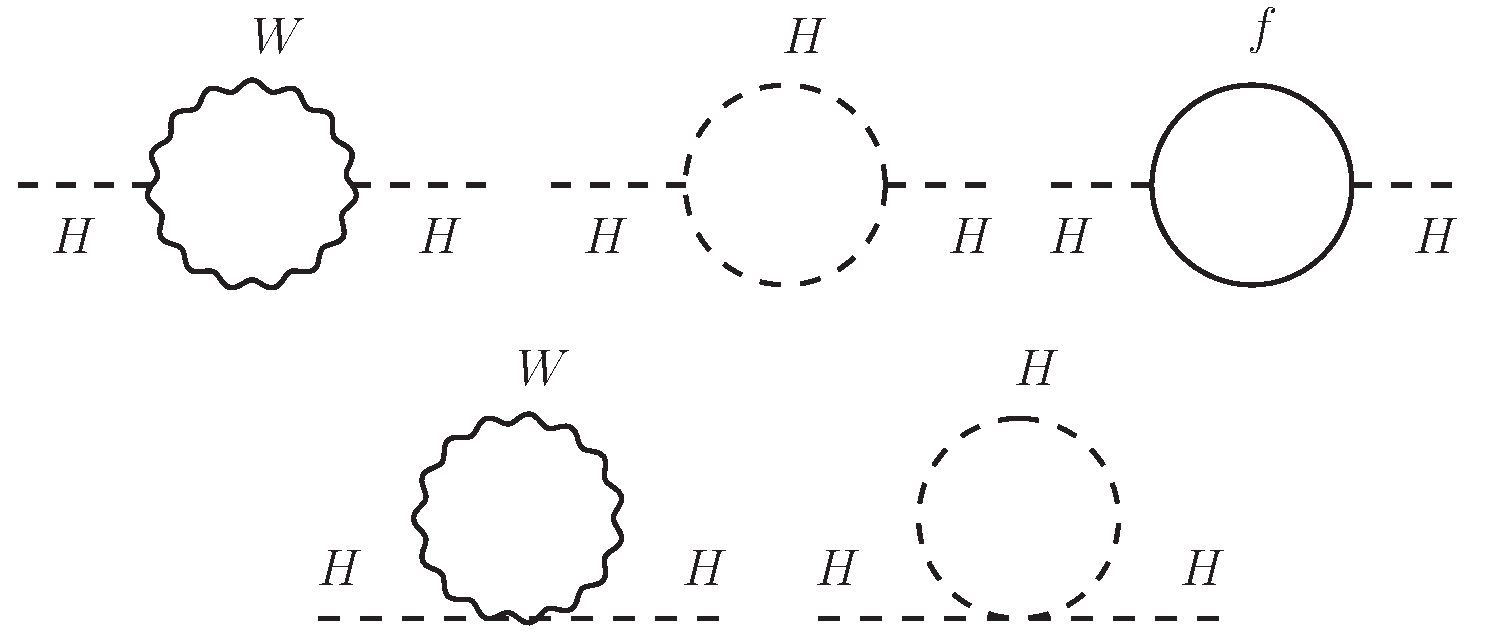
\includegraphics[scale=0.5]{figures/theory/Higgs_Virtual.pdf}
\caption[Radiative corrections to the Higgs mass]{Radiative corrections to the Higgs mass.}
\label{higgsVirtual}
\end{figure}

The Higgs mass receive quantum corrections from loops that contain bosons ($W,Z$, Higgs) and fermions (quarks and leptons), with the last one being dominated by the top quark since its contribution goes with the square of the fermion mass. Taking into account those contributions we can write the renormalized Higgs mass as, \cite{Quigg:2009vq}
\begin{equation}
\underbrace{M_H^2}_{\rm physical} = \underbrace{M_{0,H}^2}_{\rm bare}  + \quad\Lambda^2\underbrace{\left( 6M_W^2 + 3M_Z^2 + M_H^2 - 12 M_{\rm top}^2\right) \frac{G_F}{4\pi^2\sqrt{2}}}_{\text{loop corrections}}  
\label{correction}
\end{equation}
where $\Lambda$ is the maximum energy for which the SM applies, or in other words, for energies larger than $\Lambda$ a new theory should be taken into account. 

In principle, this scale can be as large as the Planck scale , that is,
\begin{equation*}
\Lambda\sim M_{\rm Planck} = \left(\frac{\hbar c}{G_{\rm Newton}}\right)^{1/2} \approx 1.2\times 10^{19}\:{\rm GeV} \; .
\end{equation*}

According to Eq. \ref{correction}, the quantum correction goes like $\Lambda^2$ and it contains the sum of the effect of the bosons loops minus the sum of the effect of the fermions loop. It is important to notice that the quantum correction is not proportional to the Higgs mass itself. Therefore, the correction is present even for a Higgs with zero bare mass. 

\begin{figure}[h]
\centering
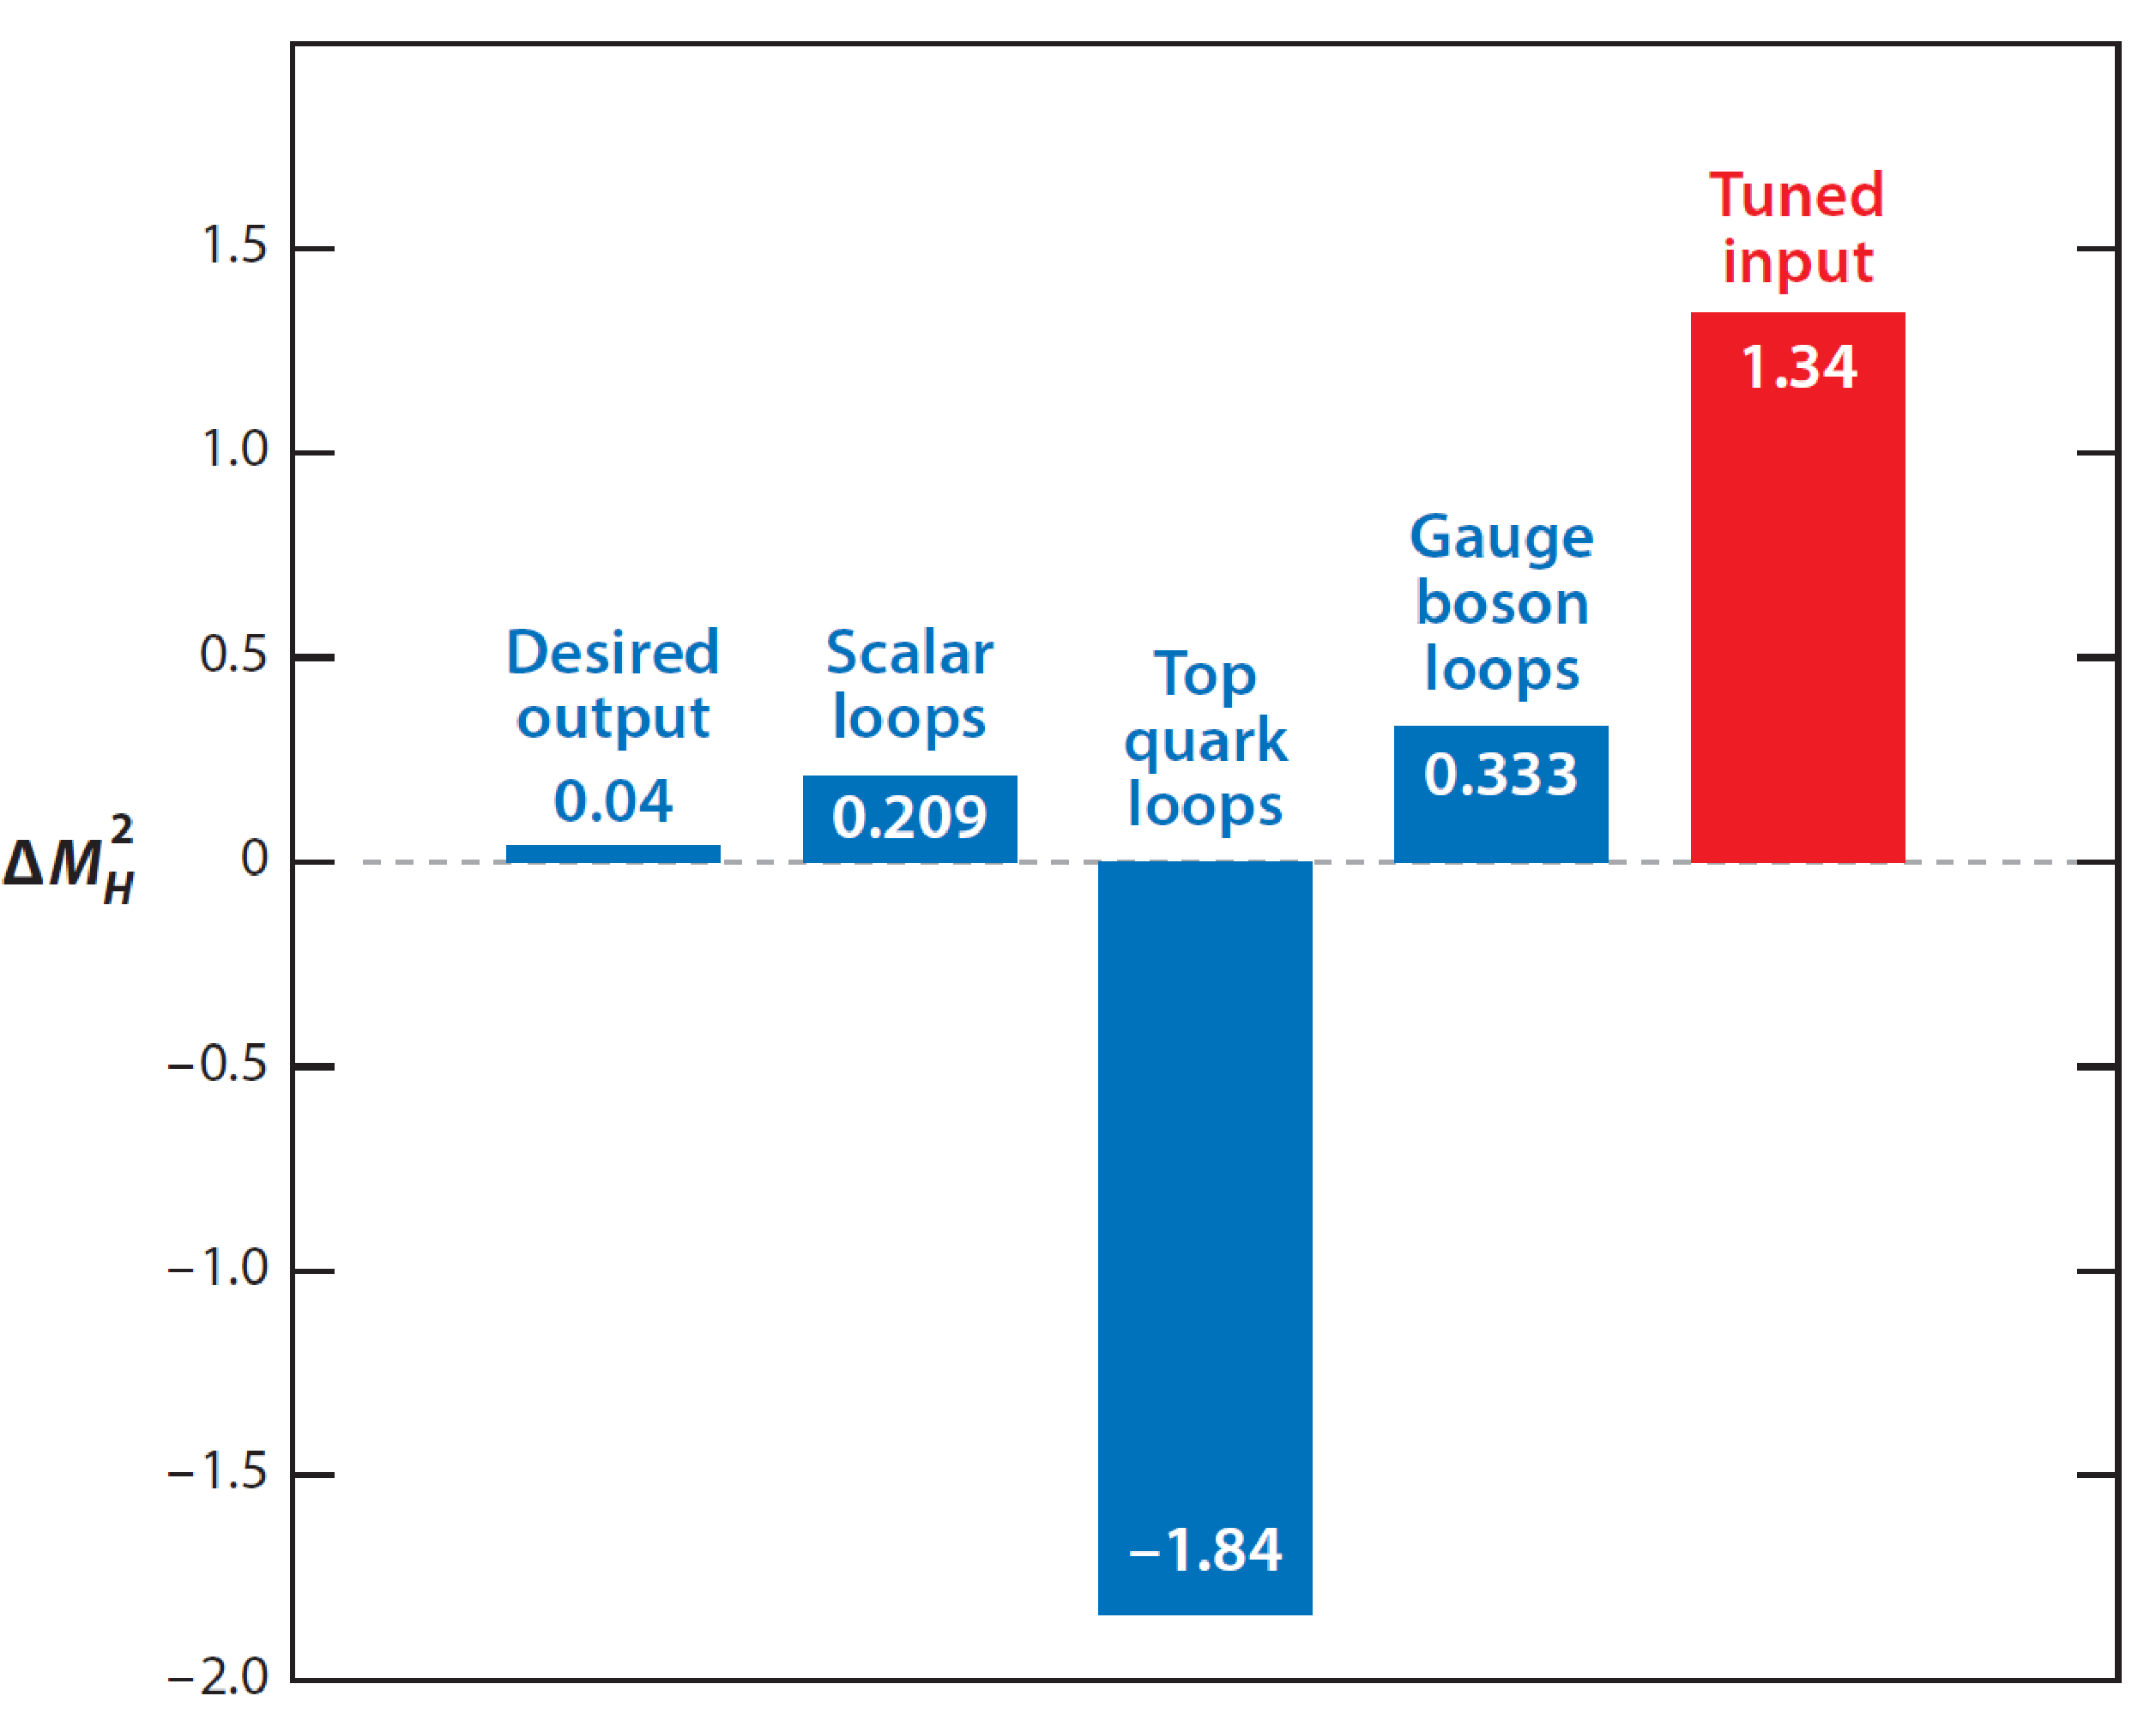
\includegraphics[scale=0.23]{figures/theory/deltaMass.pdf}
\caption[Relative contributions to $\Delta M_{H}^2$]{Relative contributions to $\Delta M_{H}^2$ for a value of $\Lambda=5$ TeV \cite{Quigg:2009vq}.}
\label{deltaMass}
\end{figure}

The physical Higgs mass  is equal to the bare mass plus a very large number ($\Lambda^2$) multiplied by a (negative) loop factor. Therefore, in order to obtain a reasonable value for the physical Higgs mass (125 GeV), the theory must have a very fine-tuning cancellation between the radiative correction and the bare mass. Even when the scale is not extremely large ($\Lambda \simeq 5$ TeV), a careful balancing is required to maintain a small Higgs mass (Fig \ref{deltaMass}).
 
Unless we suppose that the bare mass and the quantum corrections are finely tuned to yield $M_H\sim 125$ GeV, some new physics must intervene. Such precise balancing is utterly unnatural in physics theories, leading the physicists to propose a series of ways in which this cancellation could occur naturally. For instance, supersymmetry\cite{Martin:1997ns} exploits the fact that fermion loops contribute with an overall minus sign relative to the boson loops (because of Fermi statistics), balancing the contributions of fermion and boson loops. In unbroken supersymmetry, the masses of bosons are degenerate with those of their fermion counterparts, so the cancellation is exact.

\section{Beyond the Standard Model}

The standard model is in very good agreement with all experimental data obtained so far. Some of the remarkable evidences include:

\begin{compact_itemize}
	\item Existence of quarks with spin $1/2$ and gluons with spin 1, from deep-inelastic scattering experiments at SLAC (1970) and tree-jet events at DESY (1979); 
	\item Discovery of $J/\psi$ at BNL and SLAC (1974);
	\item Weak neutral current process mediated by Z bosons discovered at CERN (1973) and Fermilab (1974); 
	\item Existence of the color quantum number from different measurements: $R$, $\pi^0$ decay into photons,  anomaly cancelation, etc.; 
	\item Discovery of $W^\pm$ and $Z^0$ at CERN (1983);
	\item Discovery of the $\tau$ at SLAC (1975), $\Upsilon$ (b quark) at Fermilab (1977) and the top quark at Fermilab (1995);
	\item Precise measurement of the $Z^0$, triple vector boson interaction, and the establishment of 3-family scenario at LEP (90's);
	\item Discovery of the Higgs boson, CERN (2012).
\end{compact_itemize}

Despite this great success, some versions of the so-called physics beyond the standard model (BSM) theories \cite{Allanach:2006fy} have been proposed with the motivation of solving the fine-tuning associated with the quadratic divergence in the Higgs mass \cite{Bustamante:2009us}. These proposals involve, for instance, the supersymmetric models (SUSY) \cite{Martin:1997ns} and various forms of dynamical symmetry breaking and little Higgs models \cite{Ellis:2009su}. Some versions of theories with large extra dimensions \cite{Csaki:2004ay}, which allow the $W/Z$ bosons to propagate freely in the extra dimensions, giving rise to Kaluza-Klein \cite{Dienes:2002hg} excitations. Such excitations can also occur in the Randall-Sundrum models \cite{Randall:1999ee} and have motivated several experimental searches \cite{Chatrchyan:2012rva,Khachatryan:2014hpa,Khachatryan:2014gha,Khachatryan:2015ywa,Khachatryan:2016cfa,Khachatryan:2016sey}. 

Several aspects of the physics beyond the standard model are being explored by the LHC at the TeV scale. The B2G (Beyond 2 Generations) analysis group in CMS covers models of new physics featuring the decay of new resonances to heavy standard model objects such as top, $W$,  $Z$, or Higgs bosons. The B2G group maintains synergy with other analyses in TOP, SUSY, and EXO (exotica) physics groups. A summary of the main B2G searches is presented in Fig. \ref{B2Gsummary} which shows the observed limits at 95\% C.L. for the production of vector--like quarks, resonances decaying into heavy quarks and into a pair of vector bosons, and the search for excited quarks. The search for new physics phenomena is the one of the most important items of the LHC agenda during the next years of scheduled operation.

\begin{figure}[htb!!]
\centering
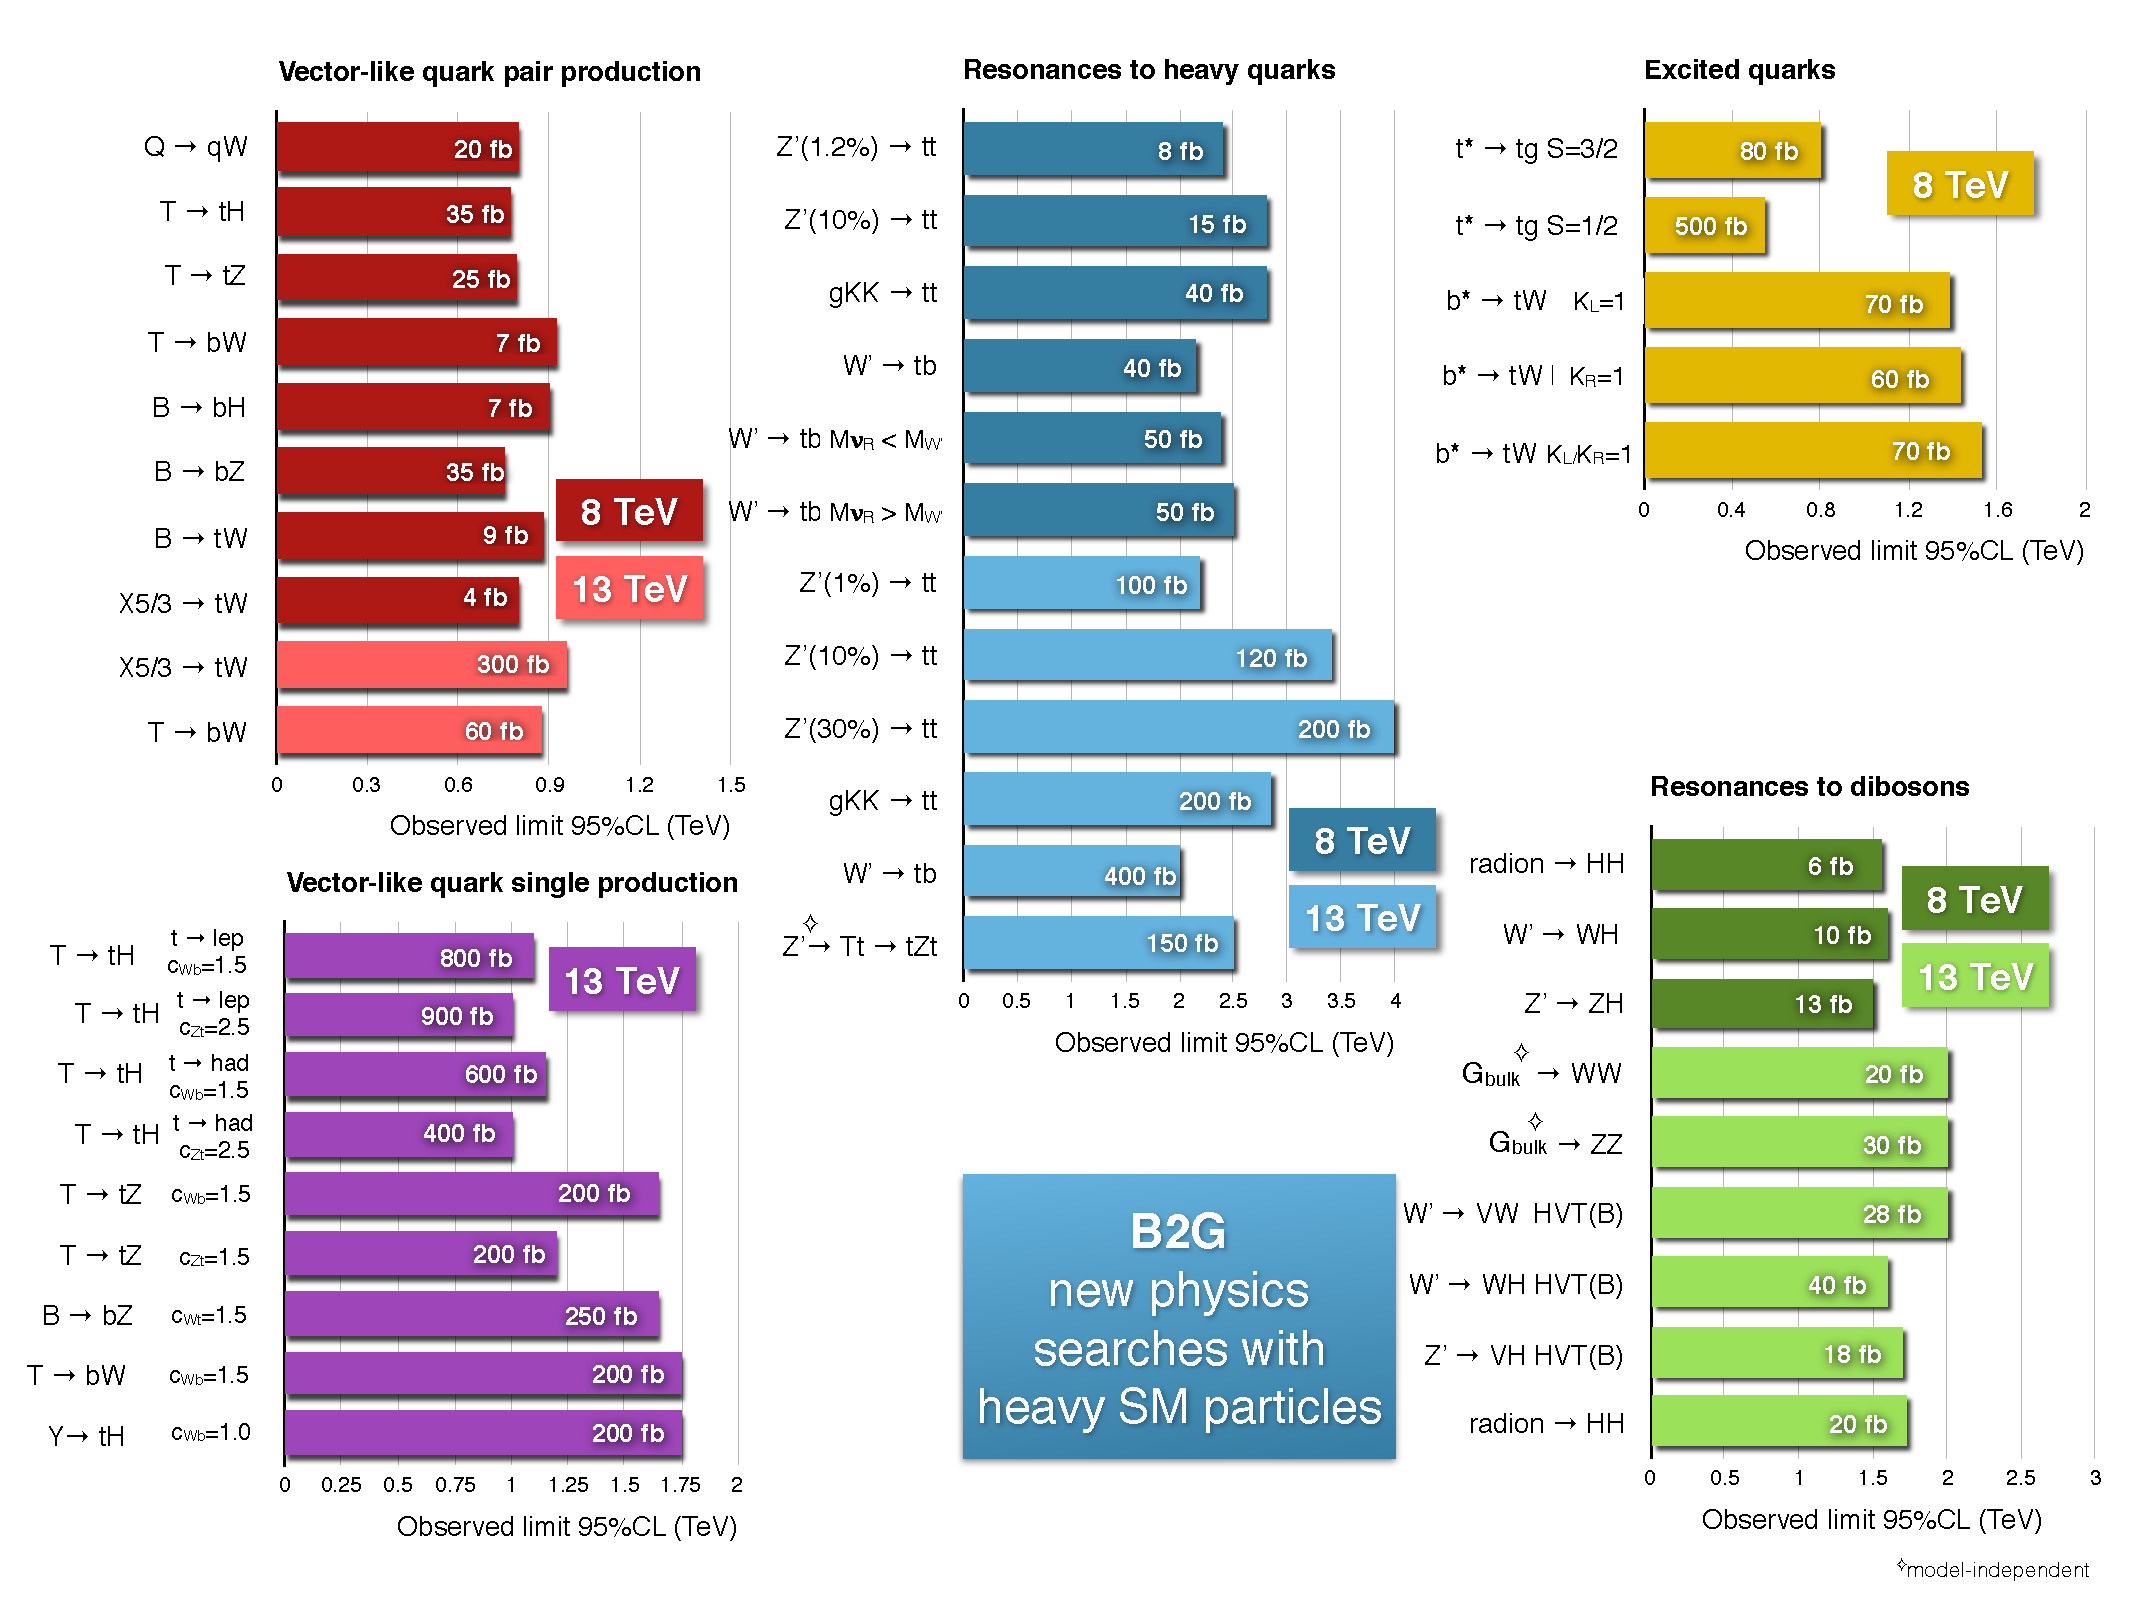
\includegraphics[scale=0.58, angle=90]{figures/theory/B2GSummary.pdf}
\caption[B2G Summary]{Summary of B2G group public physics results \cite{CMS:B2Gsummary}.}
\label{B2Gsummary}
\end{figure}

\subsection{Extra Dimensions}

An increasing number of experimentalists are actively exploring the possibility that extra spacetime dimensions might be discovered at the LHC  \cite{Csaki:2004ay}. Despite the energy scales associated to many models are considered unreachable, the examination of curled-up spacetime dimensions is directly testable. We explore here some general properties of extra spacetime dimensions starting from the original Kaluza-Klein theory formulated back in the 1920's \cite{Kaluza:1921tu}. 

The Kaluza-Klein argument provides a way of unifying particles with different spins. Certain combinations of different particles with different spins in four dimensions can be viewed as different components of a single particle in higher dimensions, with a spin associated with the higher-dimensional Lorentz group. As an example consider a vector field in five dimensions $V^{(5)} = (V_0, V_1, V_2, V_3, V_4)$. The first four dimensions can be identified as the usual four-dimensional spacetime --- $V^{(4)} = (V_0, V_1, V_2, V_3)$  --- and the remaining component as a scalar $\phi = V_4$. Thus, a single Lorentz vector representation in five dimensions has yielded both a spin-1 particle and a spin-0 particle in four dimensions. 

%The case considered by Kaluza and Klein is more elaborated than the above example, as it is sketched in Fig. \ref{kkobs}. While a spin-two symmetric tensor field $g_{\mu\nu}^{(4)}$ is interpreted as the four-dimensional graviton, a spin-one massless vector field $A_\mu^{(4)}$ is interpreted as a photon. 

%\begin{figure}[htb!!]
%\centering
%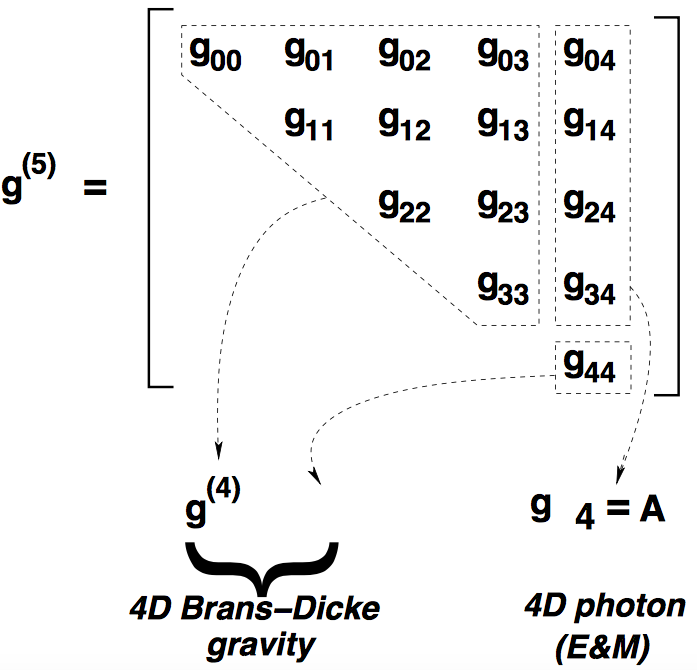
\includegraphics[scale=0.25]{figures/theory/kkobs.png}
%\caption[Basic Kaluza-Klein]{Four-dimensional Brans-Dicke gravity and four-dimensional electromagnetism can be unified within five-dimensional gravity \cite{Csaki:2004ay}.}
%\label{kkobs}
%\end{figure}

Four-dimensional gravity can indeed be unified with electromagnetism into five-dimensional gravity. While this approach succeeds in unifying both fundamental forces known in the 1920's, now we know that there are at least four fundamental interactions. Therefore, unification along these lines would require even more extra dimensions.

If any extra space dimensions exist they must be sufficiently small in order not to be observable. In other words, they must be compactified down to a small length scale. For instance, consider at every point in spacetime an additional circle of radius \textsf{\textit{R}} orthogonal to all of the known dimensions as it is illustrated in Fig. \ref{circle}. If \textsf{\textit{R}} is sufficiently small,  the extra dimension is essentially unobservable.

\begin{figure}[htb!!]
\centering
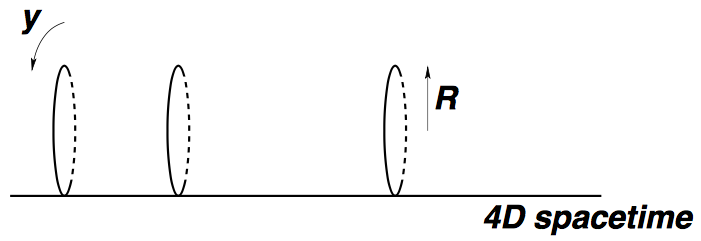
\includegraphics[scale=0.30]{figures/theory/circle.png}
\caption[Circle compactification]{Extra dimension compactified on a circle of radius $R$.}
\label{circle}
\end{figure}

More generally, the compactification of $\delta$ extra spacetime dimensions can be achieved by a theory on $\mathcal{M}_4\times K$ where $\mathcal{M}_4$ is the four-dimensional Minkowski spacetime and $K$ is any $\delta$-dimensional compact manifold. For $\delta=2$, $K=T_2$ --- a two-torus --- or $K = S_1 \times S_1$, two orthogonal circles, one for each compactified dimension. Many other topologies include manifolds with boundaries, for instance, a two-dimensional rectangle and the surface of a cylinder. A manifold with special points such as endpoints or boundaries is called orbifold.

\subsection{The Randall-Sundrum Model}
Beyond the basic idea of flat extra dimensions, deep phenomenological implications are achieved by expanding the compactification procedure to orbifolds. The proper construction of an orbifold begins with a manifold $K$ and a discrete symmetry $\Gamma$. The resulting quotient space $K/\Gamma$ is the orbifold. 

As an example, consider the circle $S^1$ satisfying the periodic boundary condition $y \leftrightarrow y + 2\pi R$. When the circle is restricted by the discrete $Z_2$ symmetry $\Gamma: y\leftrightarrow -y $, the result is a line segment identified as the orbifold $S^1 / Z_2$ (Fig. \ref{orbifold}). 

\begin{figure}[htb!!]
\centering
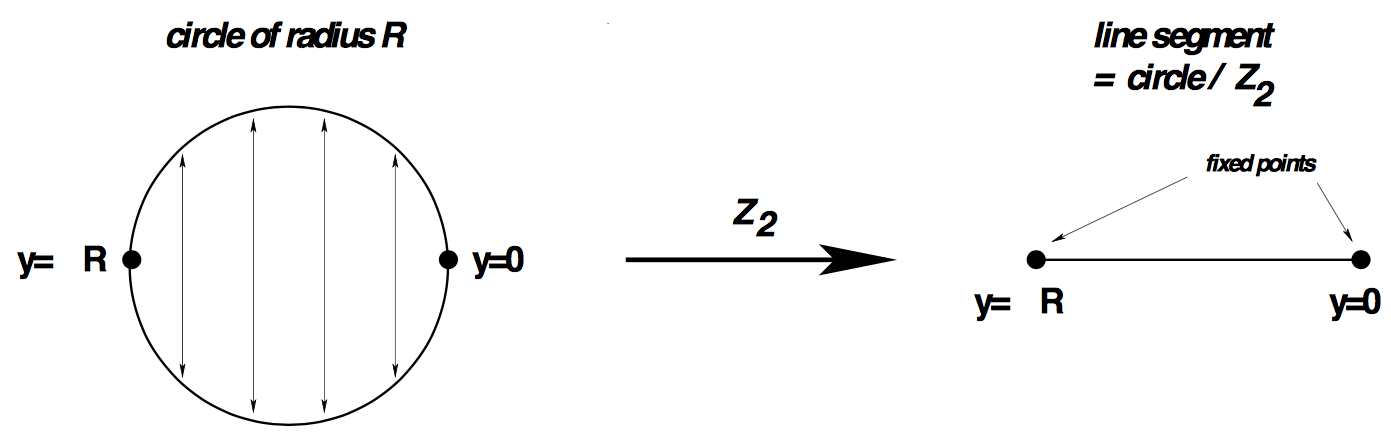
\includegraphics[scale=0.25]{figures/theory/orbifold.png}
\caption[Orbifold process]{The orbifolding process of the circle $S^1$ subjected to $Z_2$, resulting in the line segment $S^1/Z_2$.}
\label{orbifold}
\end{figure}

The compactification scheme allows to describe the extra dimension as a line segment between two four dimensional branes, known as Planck and TeV brane (Fig. \ref{branes}).

\begin{figure}[htb!!]
\centering
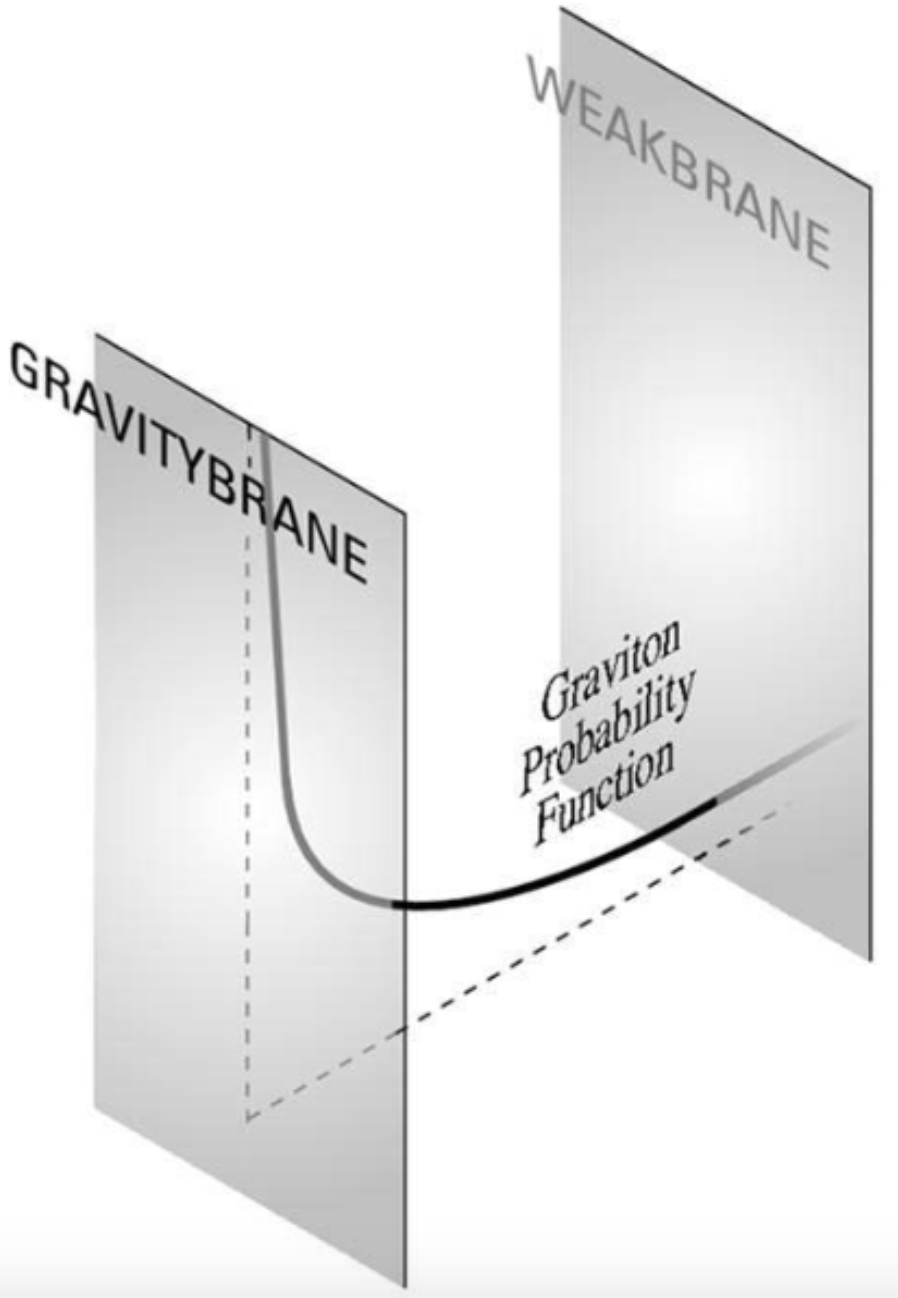
\includegraphics[scale=0.33]{figures/theory/branes.png}
\caption[Gravity and weak branes]{The Gravity (Planck) and Weak (TeV) branes are 4-dimensional boundaries of the extra dimension $y$.}
\label{branes}
\end{figure}

The Randall-Sundrum (RS) model \cite{Randall:1999ee,Randall:1999vf} is a concrete framework of warped extra dimensions. As for the extra dimension, it considers the orbifold $S^1/Z_2$, and at every point along the extra dimension, it considers the ordinary flat 4-dimensional Minkowski metric plus a fifth coordinate $y$. 

The metric satisfying these properties can be written as
\begin{equation}
ds^2 = e^{-A(y)} \, \eta_{\mu\nu} \, dx^\mu \, dx^\nu  - dy^2\,.
\end{equation}
The amount of curvature along the extra dimension depends on the function $e^{-A(y)}$, which is the warping factor. The procedure to find the solution for the function $A(y)$ involves the introduction of the curvature factor
\begin{equation}
k^2 = -\frac{\Lambda_5}{12 M^3_*}\,,
\end{equation}
relating the bulk cosmological constant $\Lambda_5$ and the 5-dimensional Planck scale $M_*$. The bulk cosmological constant \cite{Csaki:2004ay} comes from the 5-dimensional Einstein action for gravity and it has units of mass to the fifth power, $[\Lambda_5]=M^5$; therefore, the curvature factor has units of mass, $[k] = \big(M^5/M^3\big)^{1/2} = M$. Furthermore, a solution of the Einstein equation can only exist if the bulk cosmological constant is negative $\Lambda_5 < 0$. 

According to the RS model, the effective scale of gravity --- that is the 4-dimensional Planck scale --- is found to be
\begin{equation}
M^2_{Pl} = M^3_* \int_{y=-r_c}^{y=r_c} e^{-2k|y|} \, dy = \frac{M^3_*}{k} \left(1 - e^{-2kr_c} \right) \,.
\end{equation}
For large values of the compactification radius $r_c$, the 4-dimensional Planck scale barely depends on the size of the extra dimension. This means that an exponential hierarchy between the weak and the Planck scales is naturally introduced, providing a solution to the hierarchy problem of the standard model.

\subsection{Bulk Graviton Model}
The solution to the hierarchy problem of the standard model through the Randall-Sundrum model with a warped extra dimension  invokes the existence of new particles at the TeV scale. A key feature of the bulk graviton model \cite{Agashe:2007zd} is the propagation of the standard model fields in the extra dimension. As such, the standard model particles are identified with the zero-modes of the 5-dimensional fields. Provided that the new resonances have non-negligible coupling to the standard model particles, new signals might be observed at the LHC. Spin-2 gravitons, whose masses and couplings are set by the TeV scale, would appear in experiments as widely separated resonances. 

The bulk graviton extension of the original Randall-Sundrum model predicts a highly enhanced branching ratio of gravitons decaying to vector boson while suppressing the light fermions and photons channels. The production of bulk gravitons from gluon fusion and their decay into vector bosons $W/Z$ can be significant. 

The golden channel in the bulk graviton model is $G\rightarrow Z_L Z_L$, where $Z_L$ indicates the longitudinal component of the vector boson. The partial decay width of this channel is given by
\begin{equation}
\Gamma(G\rightarrow Z_L Z_L) \approx \frac{(c \, x_n^G)^2 \, m^G_n}{960 \pi}\,,
\label{larg:grav}
\end{equation}
where $c\equiv k/\overline{M}_{Pl}$, and the roots of the Bessel function of order 1, $x^G_n = $ 3.83, 7.02, 10.17, 13.32, give the masses of the first 4 Kaluza-Klein gravitons:
\begin{equation}
m^G_n = k \; e^{-k\pi R} \; x^G_n\,,
\end{equation}
where $k$ is the curvature scale and $R$ is the proper size of the extra dimension.

The production cross section for the bulk graviton with $k/M_{Pl} = 0.1$ is shown in Fig. \ref{bulkgrav}. These calculations where obtained with MG5\_aMC@NLO \cite{Alwall:2011uj} as reported in Ref. \cite{Oliveira:2014kla}. The natural width of a bulk graviton with these characteristics is less than 0.1\% of its mass, which is negligible with respect to the experimental detector resolution. For the experimental analysis we will use simulated samples with $k/M_{Pl} = 0.5$, increasing the graviton width to 1.5\%. 

\begin{figure}[htb!!]
\centering
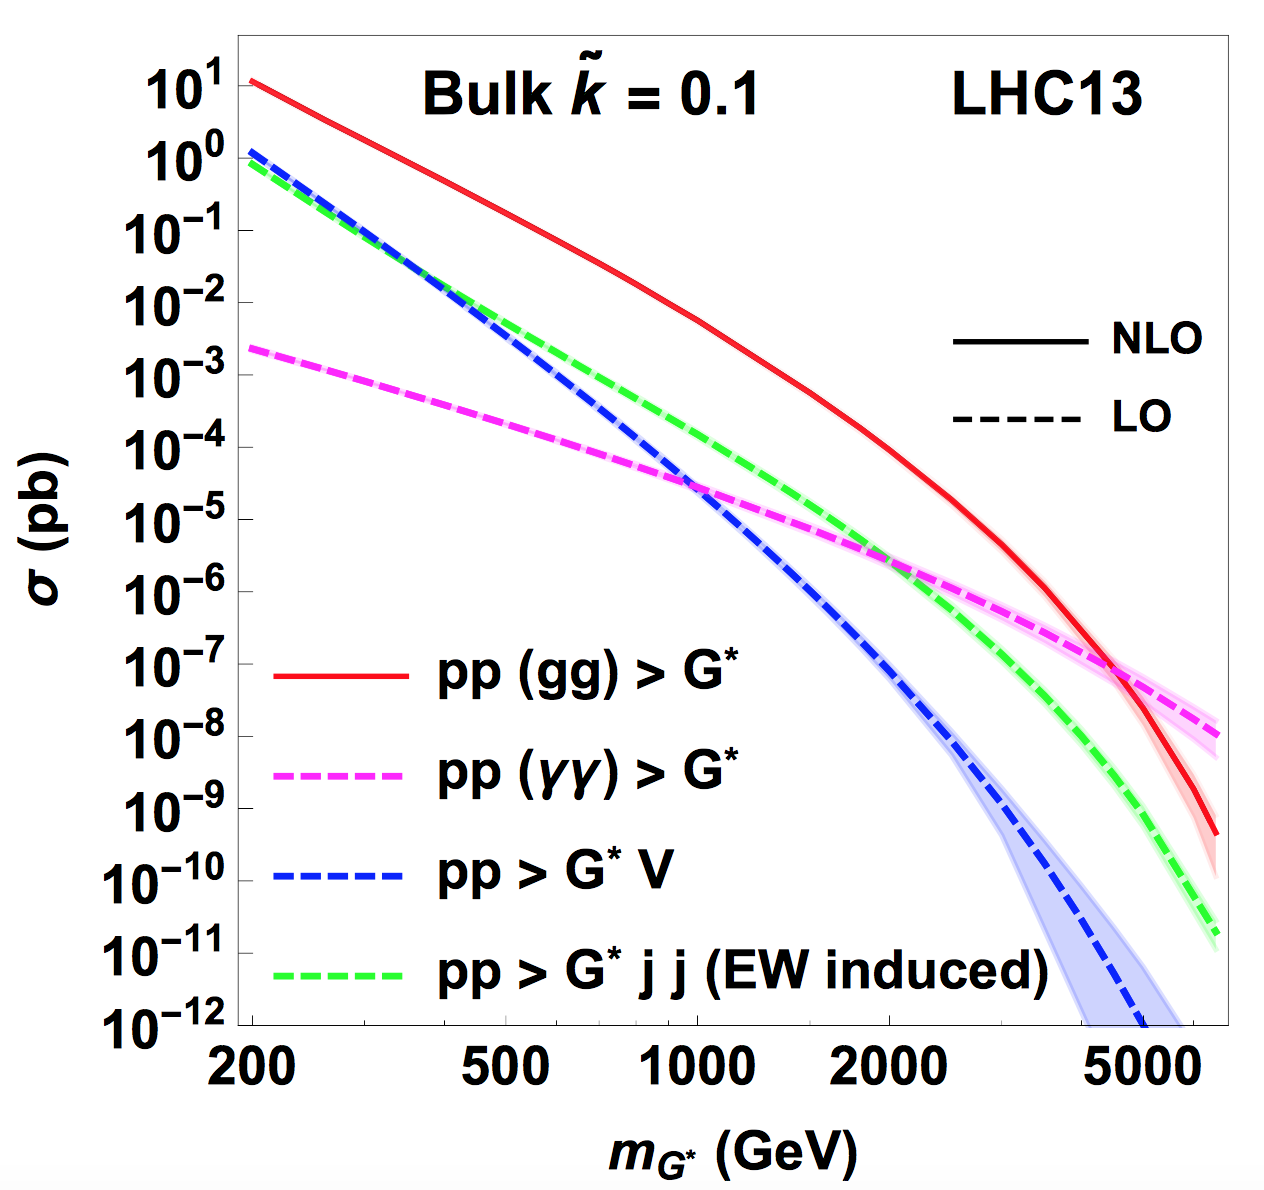
\includegraphics[width=0.75\textwidth]{figures/theory/bulkgrav.png}
\caption[Bulk Graviton cross section]{Production cross section for the bulk graviton scenario \cite{Oliveira:2014kla}. The red curve corresponds to the inclusive production, the green curve to the associated production with two jets, the blue curve to the associated production with a vector boson, and the magenta curve to the photon-fusion production. NLO (LO) calculations are shown in continuous (dashed) lines.} 
\label{bulkgrav}
\end{figure}

The most stringent limits to date on the bulk graviton signal strength are shown in Fig. \ref{latestLimits}, in the mass range 0.6 to 4.0 TeV. As observed in the figure, the sensitivity arises mainly from the 4q and 2q$\ell\nu$ channels.

\begin{figure}[htb!!]
\centering
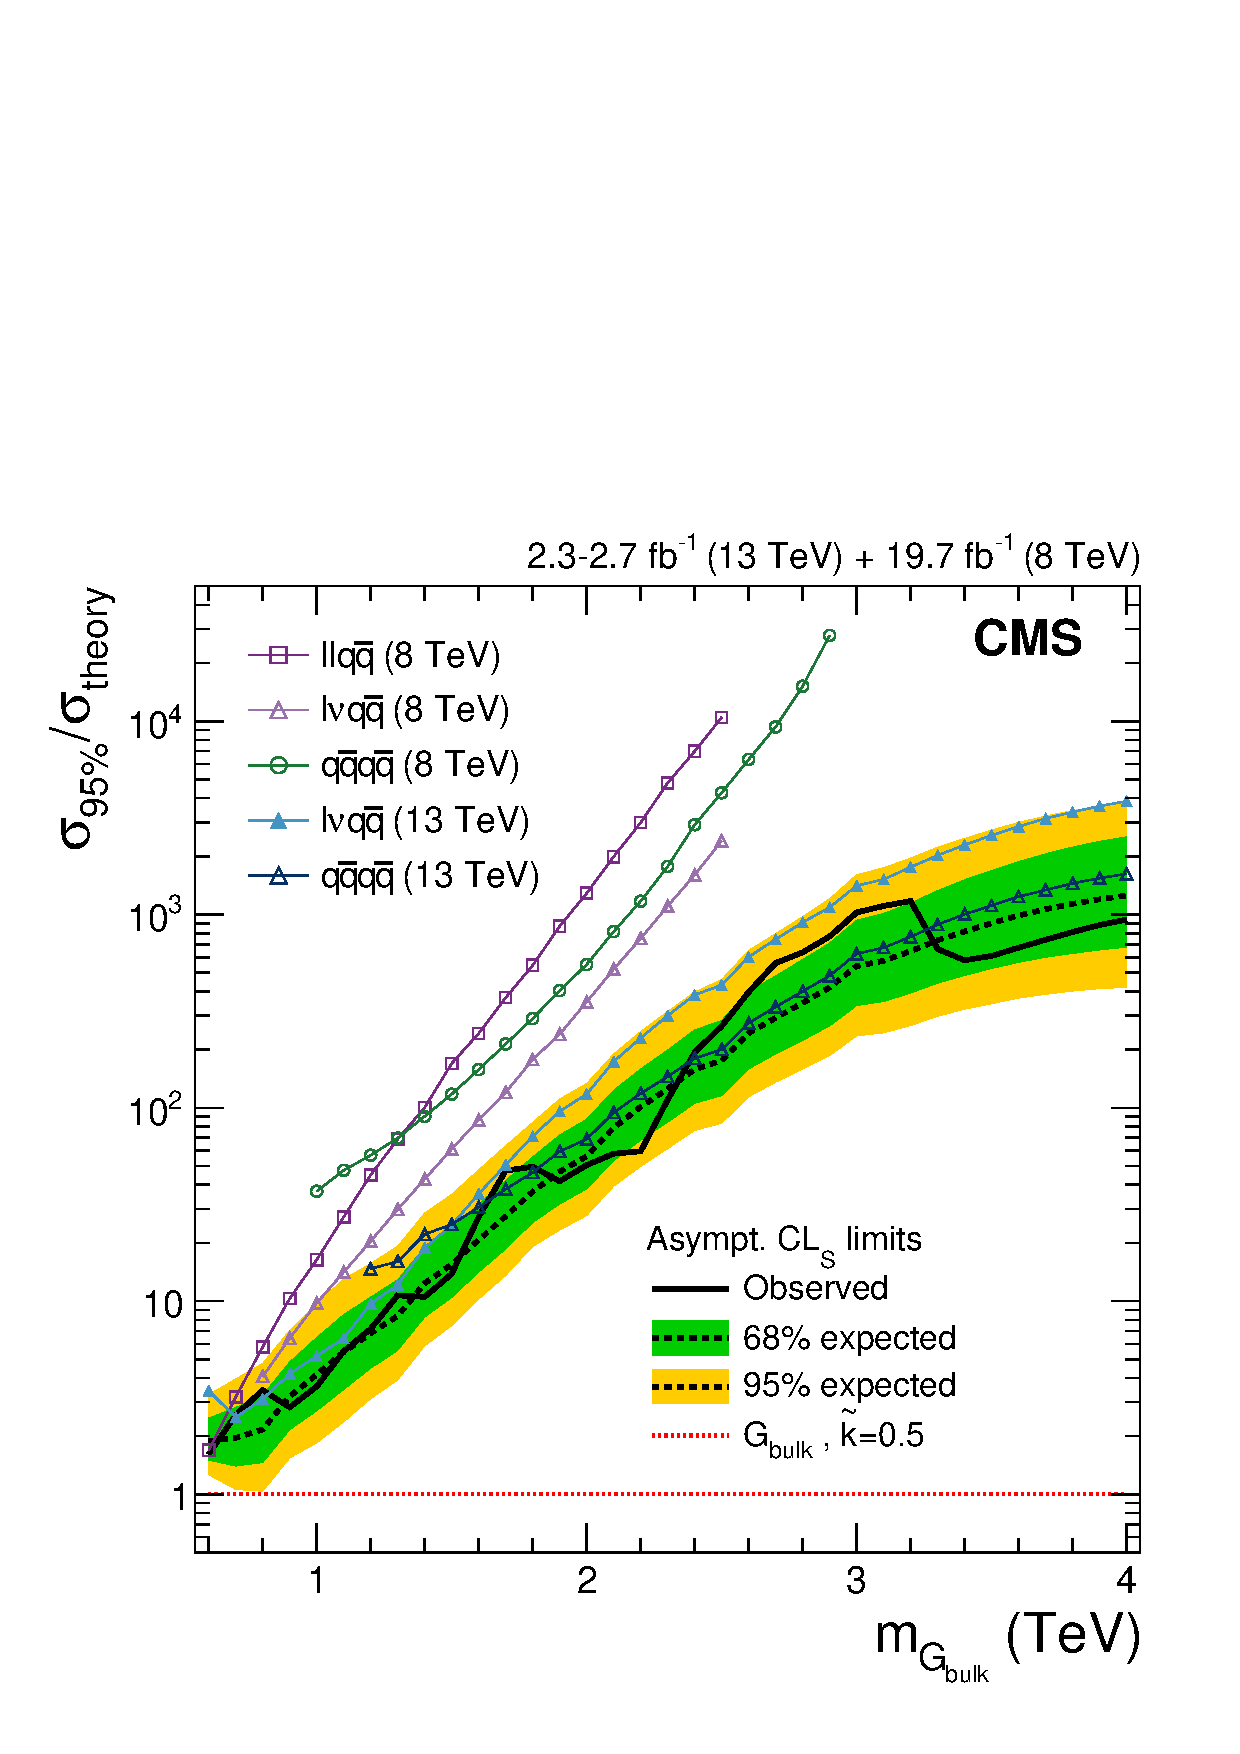
\includegraphics[width=0.85\textwidth]{figures/theory/CMS-B2G-16-007_Figure_003.pdf}
\caption[Latest limits]{Exclusion limits at 95\% CL on the signal strength in the bulk graviton model with $\tilde{k}=0.5$, as function of the resonance mass, obtained by combining 8 and 13 TeV diboson searches \cite{Sirunyan:2017nrt}.}
\label{latestLimits}
\end{figure}
